\documentclass[11pt,openany,a4paper]{article}
\usepackage{amsmath, amsfonts, amsthm, amssymb}
\usepackage{tikz, pgfplots, tkz-euclide,calc}
    \usetikzlibrary{patterns,decorations,shapes.arrows,arrows.meta}
\usepackage{fancyhdr}
\usepackage{enumerate,enumitem}
\usepackage{cancel}
\usepackage{varwidth}
\usepackage{array}
\usepackage{animate}
\usepackage{multirow,multicol}
\usepackage{hyperref}
\hypersetup{
    colorlinks=true,
    linkcolor=blue,
    filecolor=magenta,      
    urlcolor=cyan,
    pdftitle={Overleaf Example},
    pdfpagemode=FullScreen,
    }
\usepackage{graphicx}
\graphicspath{{D:/Hada Touya/Asisten-things/Asisten Dosen/PPT Kalkulus/Gambar & Logo/}{C:/Users/teoso/OneDrive/Documents/Asisten Dosen & Lab/Asisten Laboratorium/Alpro 1/PPT/Graphicx/}{C:/Users/teoso/OneDrive/Documents/Tugas Kuliah/Template Math Depart/}}

% TAMBAHKAN PACKAGE SENDIRI KALAU KURANG

\usepackage{geometry}
\geometry{
	left = 20mm,
	right = 20mm,
	top = 30mm,
	bottom = 30mm,
}


\pagestyle{fancy}
\fancyhead{}
\fancyfoot{}
\fancyhead[r]{}
\fancyhead[l]{\fbox{\large{\textbf{SKPB - ITS}}}}
\renewcommand{\headrulewidth}{0pt}
\renewcommand{\footrulewidth}{0pt}

\newcommand{\R}{\mathbb{R}}
\newcommand{\N}{\mathbb{N}}
\newcommand{\C}{\mathbb{C}}
\newcommand{\Z}{\mathbb{Z}}
\newcommand{\Q}{\mathbb{Q}}
\newcommand{\cis}{\text{cis}}

\begin{document}

\begin{center}
    {\underline{\textbf{\MakeUppercase{Evaluasi Tengah Semester Bersama Genap 2024/2025}}}}
\end{center}

\begin{center}
    \begin{tabular}{lcl}
        Mata kuliah/SKS & : & Kalkulus 1 ( SM234101 ) / 3 SKS \\
        Hari, Tanggal   & : & Kamis, 17 Oktober 2024          \\
        Waktu           & : & 07.00-08.40 WIB (100 menit)     \\
        Sifat           & : & Tertutup                        \\
        Kelas           & : & 5-12, 101
    \end{tabular}
\end{center}

\noindent\rule{\textwidth}{2.pt}

\setlength{\parindent}{5pt}
\setlength{\parindent}{5pt}
\centering{Tuliskan: Nama, NRP, dan Nomor Kelas pada lembar jawaban Anda.}
\setlength{\parindent}{5pt}
\par \textbf{\small\MakeUppercase{dilarang membawa/menggunakan kalkulator dan alat komunikasi}}
\centering{\textbf{\MakeUppercase{dilarang memberikan/menerima jawaban selama ujian}}}
\par \centering{\textbf{"Setiap tindak kecurangan akan mendapat sanksi akademik."}}
\noindent\rule{\textwidth}{2.pt}

\begin{table}[h]
    \centering
    ETS Mengukur Kemampuan
    \begin{tabular}{|c|m{11cm}|c|c|}
        \hline
        CPL & CPMK                                                                                      & SOAL & BOBOT (\%) \\ \hline
        \multirow{5}{*}{2}
            & CPMK-1 Mampu menyelesaikan persamaan dan pertidaksamaan serta menssketsa grafik persamaan & 1    & 20         \\ \cline{2-4}
            & \multirow{4}{*}{CPMK-2 Mampu menentukan kekontinuan fungsi dan turunannya}                & 2    & 20         \\\cline{3-4}
            &                                                                                           & 3    & 20         \\ \cline{3-4}
            &                                                                                           & 4    & 20         \\ \cline{3-4}
            &                                                                                           & 5    & 20         \\ \hline
    \end{tabular}
\end{table}
{\centering\textbf{SOAL}}
% SOAL DI SINI YAA
\begin{enumerate}
    \item Dapatkan himpunan penyelesaian dari
          \[
              \frac{1}{x+2} < \frac{1}{4-x}.
          \]

    \item Diberikan $f(x) = x^2 + 2,\; x \geq 0$ dan $g(x) = \sqrt{x-3}$.
          \begin{enumerate}
              \item Dapatkan domain $f(x)$ dan $g(x)$.
              \item Dapatkan $(g \circ f)(x)$ dan domain $(g \circ f)(x)$.
          \end{enumerate}

    \item Diketahui $f(x) = x^3 - 2$.
          \begin{enumerate}
              \item Dapatkan $f^{-1}(x)$ beserta domainnya.
              \item Sketsa grafik dari $f(x)$ dan $f^{-1}(x)$ pada satu bidang koordinat.
          \end{enumerate}

    \item Hitunglah $\displaystyle\lim_{x \to -\infty} \frac{\sqrt{5x^2 - 2}}{x+3}$.

    \item Dapatkan persamaan garis singgung kurva $xy^2 + y + \sqrt{x} = x + 3$ di titik $(4,1)$.
\end{enumerate}

\fancyfoot{\begin{center}
        \rule{0.28\textwidth}{2.pt}$\quad$\textbf{Selamat Mengerjakan}$\quad$\rule{0.28\textwidth}{2.pt}
        \begin{quote}
            \centering
            \textit{``Jujur adalah kunci kesuksesan''}
        \end{quote}
    \end{center}}


\newpage
\fancyhead[L]{\textit{Solution By: \hyperlink{https://github.com/TetewHeroez}{Tetew}}}
\fancyfoot{}
% \fancyfoot[R]{\animategraphics[autoplay,loop,width=0.1\textwidth]{15}{Kuru Kuru Herta/kuru kuru-}{0}{5}}
{\centering\textbf{SOLUSI}}
\renewcommand{\arraystretch}{1.5}
\renewcommand{\headrulewidth}{1pt}
\begin{enumerate}
    \item Pidahkan semua ruas ke kiri
          \begin{align*}
              \frac{1}{x+2}-\frac{1}{4-x}         & < 0 \\
              \iff \frac{4-x - (x+2)}{(x+2)(4-x)} & < 0 \\
              \iff \frac{2 - 2x}{(x+2)(4-x)}      & < 0 \\
              \iff \frac{1-x}{(x+2)(4-x)}         & < 0
          \end{align*}
          Diperoleh pembuat nol-nya adalah $x = 1, -2, 4$. Selanjutnya gunakan uji tanda, didapatkan
          \begin{itemize}
              \item $\displaystyle x=-3 \implies \frac{1-(-3)}{(-3+2)(4-(-3))} = \frac{4}{-7} < 0$
              \item $\displaystyle x=0 \implies \frac{1-0}{(0+2)(4-0)} = \frac{1}{8} > 0$
              \item $\displaystyle x=2 \implies \frac{1-2}{(2+2)(4-2)} = \frac{-1}{8} < 0$
              \item $\displaystyle x=5 \implies \frac{1-5}{(5+2)(4-5)} = \frac{-4}{-7} > 0$
          \end{itemize}
          Kemudian gambarkan garis bilangan sebagai berikut
          \begin{center}
              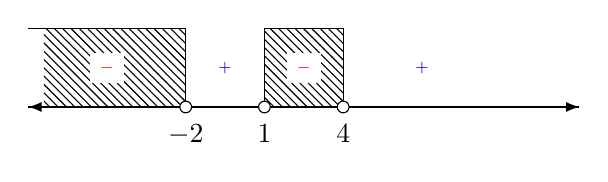
\begin{tikzpicture}
                  \draw[-Latex] (-1,0) -- (6,0);
                  \draw[Latex-] (-1,0) -- (6,0);
                  \foreach \i in {1,2,3}
                  \coordinate (A\i) at (\i,0);
                  \node[below] at ($(0,-0.1)+(A1)$) {$-2$};
                  \node[below] at ($(0,-0.1)+(A2)$) {$1$};
                  \node[below] at ($(0,-0.1)+(A3)$) {$4$};

                  \fill[lightgray,pattern=north west lines,line width=1pt](A1)rectangle($(-0.8,0)+(0,1)$);
                  \fill[lightgray,pattern=north west lines,line width=1pt](A2)rectangle($(3,0)+(0,1)$);

                  \draw (A1)--($(A1)+(0,1)$)--($(-1,0)+(0,1)$);
                  \draw (A2)--($(A2)+(0,1)$)--($(A3)+(0,1)$)--(A3);

                  \foreach \i in {1,3}
                  \node[circle,draw,fill=white,inner sep=1.5pt] at (A\i) {};
                  \node[circle,draw,fill=white,inner sep=1.5pt] at (A2) {};

                  \node[fill=white!5] at ($(A1)+(-1,0.5)$) {\tiny\color{red}$-$};
                  \node[fill=white!5] at ($0.5*(A1)+0.5*(A2)+(0,0.5)$) {\tiny\color{blue}$+$};
                  \node[fill=white!5] at ($0.5*(A2)+0.5*(A3)+(0,0.5)$) {\tiny\color{red}$-$};
                  \node[fill=white!5] at ($(A3)+(1,0.5)$) {\tiny\color{blue}$+$};

              \end{tikzpicture}
          \end{center}
          Sehingga diperoleh himpunan penyelesaian dari pertidaksamaan tersebut adalah
          \[H_p=\{x\in\R\,|\,x<-2\vee 1\geq x<4\}=(-\infty,-2) \cup (1,4).\]

    \item \begin{enumerate}
              \item Karena polinomial selalu terdefinisi di $\R$, maka domain $f$ adalah $\mathcal{D}_f = [0,\infty)$ (karena dibatasi untuk $x\geq 0$). Sedangkan untuk $g(x) = \sqrt{x-3}$, agar terdefinisi maka $x-3 \geq 0 \implies x \geq 3$. Dengan demikian, domain dari $g$ adalah $\mathcal{D}_g = [3,\infty)$.
              \item \begin{align*}
                        (g \circ f)(x)  = g(f(x))
                        = g(x^2 + 2)
                        = \sqrt{(x^2 + 2) - 3}
                        = \sqrt{x^2 - 1}
                    \end{align*}
                    Menurut definisi domain komposisi fungsi, maka
                    \begin{align*}
                        \mathcal{D}_{g \circ f} & = \{x \in \mathcal{D}_f \,|\, f(x) \in \mathcal{D}_g\}        \\
                                                & = \{x \in [0,\infty) \,|\, x^2 + 2 \in [3,\infty)\}           \\
                                                & = \{x \in [0,\infty) \,|\, x^2 + 2 \geq 3\}                   \\
                                                & = \{x \in [0,\infty) \,|\, x^2 - 1 \geq 0\}                   \\
                                                & = \{x \in [0,\infty) \,|\, x \geq 1 \text{ atau } x \leq -1\} \\
                                                & = [1,\infty).
                    \end{align*}
                    Jadi domain dari $(g \circ f)(x)$ adalah $\mathcal{D}_{g \circ f} = [1,\infty)$.
          \end{enumerate}
    \item \begin{enumerate}
              \item Tukar $y = f(x)$ menjadi $x = f(y)$, sehingga
                    \begin{align*}
                        x         & = y^3 - 2          \\
                        y^3       & = x + 2            \\
                        y         & = \sqrt[3]{x + 2}. \\
                        f^{-1}(x) & = \sqrt[3]{x + 2}.
                    \end{align*}
                    Selanjutnya kita tahu bahwa $\mathcal{D}_{f^{-1}} = \mathcal{R}_f = \R$ (karena fungsi kubik memiliki range semua bilangan real $(\R)$).
              \item Grafik $f(x)$ dan $f^{-1}(x)$ dapat digambarkan sebagai berikut
                    \begin{center}
                        \begin{tikzpicture}
                            \begin{axis}[
                                    axis lines = middle,
                                    xlabel = $x$,
                                    ylabel = {$y$},
                                    xtick={-4,-2,...,4},
                                    ytick={-4,-2,...,4},
                                    ymin=-5.5, ymax=5.5,
                                    xmin=-5.5, xmax=5.5,
                                    grid=both,
                                    width=10cm,
                                    height=10cm,
                                    grid style={line width=.1pt, draw=gray!10},
                                    major grid style={line width=.2pt,draw=gray!50},
                                    x label style={anchor=west}, % label x ke kanan
                                    y label style={anchor=south}, % label y ke atas
                                    samples=200,
                                    legend style={
                                            at={(1.1,1)},
                                            anchor=north west,
                                            font=\small,         % mengecilkan ukuran font
                                            row sep=1pt,         % jarak antar baris legend
                                            inner sep=1pt,       % margin dalam kotak legend
                                            nodes={scale=0.7}    % skalakan isi legend
                                        }
                                ]
                                \addplot[
                                    domain=-2:2,
                                    samples=200,
                                    color=blue,
                                ]
                                {x^3 - 2};
                                \addlegendentry{$f(x) = x^3 - 2$}

                                \addplot[
                                    domain=-5:5,
                                    samples=200,
                                    color=red,
                                ]
                                {sign(x+2)*abs(x+2)^(1/3)};
                                \addlegendentry{$f^{-1}(x) = \sqrt[3]{x + 2}$}

                                \addplot[
                                    domain=-5:5,
                                    samples=100,
                                    color=black,
                                    dashed
                                ]
                                {x};
                                \addlegendentry{$y=x$}
                            \end{axis}
                        \end{tikzpicture}
                    \end{center}
          \end{enumerate}
    \item Bagi pembilang dan penyebut dengan $|x|$ agar bentuknya menjadi
          \begin{align*}
              \lim_{x \to -\infty} \frac{\sqrt{5x^2 - 2}}{x+3}= \lim_{x \to -\infty} \frac{\frac{\sqrt{5x^2 - 2}}{|x|}}{\frac{x+3}{|x|}} = \lim_{x \to -\infty} \frac{\frac{\sqrt{5x^2 - 2}}{\sqrt{x^2}}}{\frac{x+3}{|x|}} = \lim_{x \to -\infty} \frac{\sqrt{5 - \frac{2}{x^2}}}{\frac{x+3}{|x|}}.
          \end{align*}
          karena $x \to -\infty$, maka $|x| = -x$. Sehingga
          \begin{align*}
              \lim_{x \to -\infty} \frac{\sqrt{5 - \frac{2}{x^2}}}{\frac{x+3}{|x|}} & = \lim_{x \to -\infty} \frac{\sqrt{5 - \frac{2}{x^2}}}{\frac{x+3}{-x}}= \lim_{x \to -\infty} \frac{\sqrt{5 - \frac{2}{x^2}}}{-1 - \frac{3}{x}} = \frac{\sqrt{5 - 0}}{-1 - 0}                                            =-\sqrt{5}.
          \end{align*}
    \item Diketahui $xy^2 + y + \sqrt{x} = x + 3$. Turunkan kedua ruas terhadap $x$,
          \begin{align*}
              \frac{d}{dx}(xy^2) + \frac{d}{dx}(y) + \frac{d}{dx}(\sqrt{x})   & = \frac{d}{dx}(x) + \frac{d}{dx}(3)              \\
              y^2 + x(2y \frac{dy}{dx}) + \frac{dy}{dx} + \frac{1}{2\sqrt{x}} & = 1 + 0                                          \\
              y^2 + 2xy \frac{dy}{dx} + \frac{dy}{dx} + \frac{1}{2\sqrt{x}}   & = 1                                              \\
              (2xy + 1) \frac{dy}{dx}                                         & = 1 - y^2 - \frac{1}{2\sqrt{x}}                  \\
              \frac{dy}{dx}                                                   & = \frac{1 - y^2 - \frac{1}{2\sqrt{x}}}{2xy + 1}.
          \end{align*}
          Selanjutnya, kita substitusi titik $(4,1)$ ke dalam turunan tersebut,
          \begin{align*}
              \left.\frac{dy}{dx}\right|_{(4,1)} & = \frac{1 - 1^2 - \frac{1}{2\sqrt{4}}}{2(4)(1) + 1} = \frac{0 - \frac{1}{4}}{8 + 1} = -\frac{\frac{1}{4}}{9} = -\frac{1}{36}.
          \end{align*}
          Dengan demikian, gradien garis singgung di titik $(4,1)$ adalah $m = -\frac{1}{36}$. Gunakan persamaan garis
          \[
              y - y_1 = m(x - x_1)
          \]
          dengan $(x_1,y_1) = (4,1)$, sehingga diperoleh
          \begin{align*}
              y - 1 & = -\frac{1}{36}(x - 4)              \\
              y     & = -\frac{1}{36}x + \frac{4}{36} + 1 \\
              y     & = -\frac{1}{36}x + \frac{40}{36}    \\
              y     & = -\frac{1}{36}x + \frac{10}{9}.
          \end{align*}
\end{enumerate}

\newpage
\renewcommand{\arraystretch}{1}
\fancyhead{}
\fancyfoot{}
\fancyhead[r]{}
\fancyhead[l]{\fbox{\large{\textbf{SKPB - ITS}}}}
\renewcommand{\headrulewidth}{0pt}
\renewcommand{\footrulewidth}{0pt}
\begin{center}
    {\underline{\textbf{\MakeUppercase{Evaluasi Tengah Semester Bersama Genap 2024/2025}}}}
\end{center}

\begin{center}
    \begin{tabular}{lcl}
        Mata kuliah/SKS & : & Kalkulus 1 ( SM234101 ) / 3 SKS \\
        Hari, Tanggal   & : & Kamis, 17 Oktober 2024          \\
        Waktu           & : & 07.00-08.40 WIB (100 menit)     \\
        Sifat           & : & Tertutup                        \\
        Kelas           & : & 13-19, 103
    \end{tabular}
\end{center}

\noindent\rule{\textwidth}{2.pt}

\setlength{\parindent}{5pt}
\setlength{\parindent}{5pt}
\centering{Tuliskan: Nama, NRP, dan Nomor Kelas pada lembar jawaban Anda.}
\setlength{\parindent}{5pt}
\par \textbf{\small\MakeUppercase{dilarang membawa/menggunakan kalkulator dan alat komunikasi}}
\centering{\textbf{\MakeUppercase{dilarang memberikan/menerima jawaban selama ujian}}}
\par \centering{\textbf{"Setiap tindak kecurangan akan mendapat sanksi akademik."}}
\noindent\rule{\textwidth}{2.pt}

\begin{table}[h]
    \centering
    ETS Mengukur Kemampuan
    \begin{tabular}{|c|m{11cm}|c|c|}
        \hline
        CPL & CPMK                                                                                      & SOAL & BOBOT (\%) \\ \hline
        \multirow{5}{*}{2}
            & CPMK-1 Mampu menyelesaikan persamaan dan pertidaksamaan serta menssketsa grafik persamaan & 1    & 20         \\ \cline{2-4}
            & \multirow{4}{*}{CPMK-2 Mampu menentukan kekontinuan fungsi dan turunannya}                & 2    & 20         \\\cline{3-4}
            &                                                                                           & 3    & 20         \\ \cline{3-4}
            &                                                                                           & 4    & 20         \\ \cline{3-4}
            &                                                                                           & 5    & 20         \\ \hline
    \end{tabular}
\end{table}
{\centering\textbf{SOAL}}
% SOAL DI SINI YAA
\begin{enumerate}
    \item Diberikan titik $A(2,-1)$, $B(2,2)$ dan $C(0,4)$. Dapatkan persamaan garis yang melalui titik $A$ dan sejajar dengan garis yang melalui $B$ dan $C$.

    \item Diberikan $f(x) = \dfrac{1}{x^2 - 4}$ dan $g(x) = \sqrt{x+1}$.
          \begin{enumerate}
              \item Dapatkan domain $f(x)$ dan $g(x)$.
              \item Dapatkan $(f \circ g)(x)$ dan domain $(f \circ g)(x)$.
          \end{enumerate}

    \item Diberikan $f(x) = x^2 - 4x + 7$.
          \begin{enumerate}
              \item Tentukan domain dari $f$ sehingga $f^{-1}$ ada.
              \item Dapatkan $f^{-1}$ beserta domainnya.
          \end{enumerate}

    \item Dapatkan nilai $k$ sedemikian sehingga fungsi
          \[
              f(x) =
              \begin{cases}
                  x^2 - k, & x < 3    \\
                  3x - 3,  & x \geq 3
              \end{cases}
          \]
          kontinu di $x=3$.

    \item Dapatkan $f'(x)$ dimana
          $
              f(x) = \sqrt{\dfrac{(3x+1)^3}{2x}}.
          $

\end{enumerate}

\fancyfoot{\begin{center}
        \rule{0.28\textwidth}{2.pt}$\quad$\textbf{Selamat Mengerjakan}$\quad$\rule{0.28\textwidth}{2.pt}
        \begin{quote}
            \centering
            \textit{``Jujur adalah kunci kesuksesan''}
        \end{quote}
    \end{center}}


\newpage
\fancyfoot{}
\fancyhead[L]{\textit{Solution By: \hyperlink{https://github.com/TetewHeroez}{Tetew}}}
% \fancyfoot[R]{\animategraphics[autoplay,loop,width=0.1\textwidth]{15}{Kuru Kuru Herta/kuru kuru-}{0}{5}}
{\centering\textbf{SOLUSI}}
\renewcommand{\arraystretch}{1.5}
\renewcommand{\headrulewidth}{1pt}
\begin{enumerate}
    \item Hitung gradien garis $BC$ dengan $B(2,2)$ dan $C(0,4)$,
          \[
              m_{BC} = \frac{y_2 - y_1}{x_2 - x_1} = \frac{4 - 2}{0 - 2} = \frac{2}{-2} = -1.
          \]
          Karena garis yang melalui titik $A$ sejajar dengan garis $BC$, maka gradiennya juga $-1$. Gunakan persamaan garis
          \[
              y - y_1 = m(x - x_1)
          \]
          dengan titik $A$ adalah $(x_1,y_1) = (2,-1)$, sehingga diperoleh
          \begin{align*}
              y - (-1) & = -1(x - 2) \\
              y + 1    & = -x + 2    \\
              y        & = -x + 1.
          \end{align*}

    \item \begin{enumerate}
              \item Agar $f(x) = \dfrac{1}{x^2 - 4}$ terdefinisi, maka $x^2 - 4 \neq 0 \implies x^2 \neq 4 \implies x \neq \pm 2$. Dengan demikian, domain dari $f$ adalah $\mathcal{D}_f = \R \setminus \{-2,2\}=\{x \in \R \,|\, x \ne -2\vee x \ne 2\}$. Sedangkan untuk $g(x) = \sqrt{x+1}$, agar terdefinisi maka $x + 1 \geq 0 \implies x \geq -1$. Dengan demikian, domain dari $g$ adalah $\mathcal{D}_g = [-1,\infty)$.
              \item \begin{align*}
                        (f \circ g)(x)  = f(g(x))
                        = f(\sqrt{x+1})
                        = \frac{1}{(\sqrt{x+1})^2 - 4}
                        = \frac{1}{x + 1 - 4}
                        = \frac{1}{x - 3}.
                    \end{align*}
                    Menurut definisi domain komposisi fungsi, maka
                    \begin{align*}
                        \mathcal{D}_{f \circ g} & = \{x \in \mathcal{D}_g \,|\, g(x) \in \mathcal{D}_f\}           \\
                                                & = \{x \in [-1,\infty) \,|\, \sqrt{x+1} \in \R\setminus\{-2,2\}\} \\
                                                & = \{x \geq -1 \,|\, \sqrt{x+1} \ne 2\}                           \\
                                                & = \{x \geq -1 \,|\, x + 1 \ne 4\}                                \\
                                                & = \{x \geq -1 \,|\, x \ne 3\}                                    \\
                                                & = [-1,3) \cup (3,\infty).
                    \end{align*}
                    Jadi domain dari $(f \circ g)(x)$ adalah $\mathcal{D}_{f \circ g} = [-1,3) \cup (3,\infty)$.
          \end{enumerate}
    \item
          \begin{enumerate}
              \item Ubah ekspresi fungsi tersebut dalam bentuk seperti berikut:
                    \begin{align*}
                        f(x) & = x^2 - 4x + 7       \\
                        f(x) & = (x^2 - 4x + 4) + 3 \\
                        f(x) & = (x - 2)^2 + 3.
                    \end{align*}
                    Selanjutnya kita akan coba gambarkan grafiknya dimana merupakan grafik $y=x^2$ yang digeser 2 satuan ke kanan dan 3 satuan ke atas.
                    \begin{center}
                        \begin{tikzpicture}
                            \begin{axis}[
                                    axis lines = middle,
                                    xlabel = $x$,
                                    ylabel = {$y$},
                                    xtick={-2,0,...,6},
                                    ytick={-1,3,...,12},
                                    ymin=-2.5, ymax=12.5,
                                    xmin=-1.5, xmax=6.5,
                                    grid=both,
                                    width=10cm,
                                    height=10cm,
                                    grid style={line width=.1pt, draw=gray!10},
                                    major grid style={line width=.2pt,draw=gray!50},
                                    x label style={anchor=west}, % label x ke kanan
                                    y label style={anchor=south}, % label y ke atas
                                    samples=200,
                                    legend style={
                                            at={(1.1,1)},
                                            anchor=north west,
                                            font=\small,         % mengecilkan ukuran font
                                            row sep=1pt,         % jarak antar baris legend
                                            inner sep=1pt,       % margin dalam kotak legend
                                            nodes={scale=0.7}    % skalakan isi legend
                                        }
                                ]
                                \addplot[
                                    color=blue,
                                    thick,
                                    dashed
                                ]
                                coordinates {(2,-2) (2,12)};
                                \addlegendentry{$x=2$}

                                \addplot[
                                    domain=-1:6,
                                    samples=200,
                                    color=red,
                                ]
                                {(x-2)^2 + 3};
                                \addlegendentry{$f(x)=(x-2)^2 + 3$}
                            \end{axis}
                        \end{tikzpicture}

                    \end{center}
                    dapat di analisis bahwa $f(x)$ mempunya invers jika dibatasi pada sumbu simetri nya yaitu $x=2$. Sehingga domain $f$ agar $f^{-1}$ ada adalah $\mathcal{D}_f = [2,\infty)$ atau $\mathcal{D}_f = (-\infty,2]$.

              \item Tukar $y = f(x)$ menjadi $x = f(y)$, sehingga
                    \begin{align*}
                        x                                & = y^2 - 4y + 7                              \\
                        x - 7                            & = y^2 - 4y                                  \\
                        y^2 - 4y                         & = x - 7                                     \\
                        y^2 - 4y + 4                     & = x - 7 + 4                                 \\
                        (y - 2)^2                        & = x - 3                                     \\
                        y - 2                            & = \pm\sqrt{x - 3}                           \\
                        y                                & = 2 \pm \sqrt{x - 3}.                       \\
                        f^{-1}(x)     = 2 + \sqrt{x - 3} & \text{ atau } f^{-1}(x) = 2 - \sqrt{x - 3}.
                    \end{align*}
                    Selanjutnya kita tahu bahwa $\mathcal{D}_{f^{-1}} = \mathcal{R}_f$. Jika kita ambil $\mathcal{D}_f = [2,\infty)$, maka $\mathcal{R}_f = [3,\infty)$ sehingga $\mathcal{D}_{f^{-1}} = [3,\infty)$ dan $f^{-1}(x) = 2 + \sqrt{x - 3}$.
                    Grafik $f(x)$ dan $f^{-1}(x)$ untuk $\mathcal{D}_f = [2,\infty)$ dan $\mathcal{D}_{f^{-1}} = [3,\infty)$ dapat digambarkan sebagai berikut:
                                    \begin{center}
                                        \begin{tikzpicture}
                                            \begin{axis}[
                                                    axis lines = middle,
                                                    xlabel = $x$,
                                                    ylabel = {$y$},
                                                    xtick={0,2,4,6,8,10},
                                                    ytick={0,3,6,9,12},
                                                    ymin=0, ymax=12.5,
                                                    xmin=0, xmax=10.5,
                                                    grid=both,
                                                    width=10cm,
                                                    height=10cm,
                                                    grid style={line width=.1pt, draw=gray!10},
                                                    major grid style={line width=.2pt,draw=gray!50},
                                                    x label style={anchor=west},
                                                    y label style={anchor=south},
                                                    samples=200,
                                                    legend style={
                                                            at={(1.05,1)},
                                                            anchor=north west,
                                                            font=\small,
                                                            row sep=1pt,
                                                            inner sep=1pt,
                                                            nodes={scale=0.7}
                                                        }
                                                ]
                                                \addplot[
                                                    domain=2:10,
                                                    samples=200,
                                                    color=blue,
                                                    thick
                                                ]
                                                {(x-2)^2 + 3};
                                                \addlegendentry{$f(x)=(x-2)^2+3$}

                                                \addplot[
                                                    domain=3:12,
                                                    samples=200,
                                                    color=red,
                                                    thick
                                                ]
                                                {2 + sqrt(x-3)};
                                                \addlegendentry{$f^{-1}(x)=2+\sqrt{x-3}$}

                                                \addplot[
                                                    domain=0:12,
                                                    samples=100,
                                                    color=black,
                                                    dashed
                                                ]
                                                {x};
                                                \addlegendentry{$y=x$}
                                            \end{axis}
                                        \end{tikzpicture}
                                    \end{center}

                                    Namun jika kita ambil $\mathcal{D}_f = (-\infty,2]$, maka $\mathcal{R}_f = (-\infty,3]$ sehingga $\mathcal{D}_{f^{-1}} = (-\infty,3]$ dan $f^{-1}(x) = 2 - \sqrt{x - 3}$.
                    Grafik $f(x)$ dan $f^{-1}(x)$ untuk $\mathcal{D}_f = (-\infty,2]$ dan $\mathcal{D}_{f^{-1}} = (-\infty,3]$ dapat digambarkan sebagai berikut:
                    \begin{center}
                        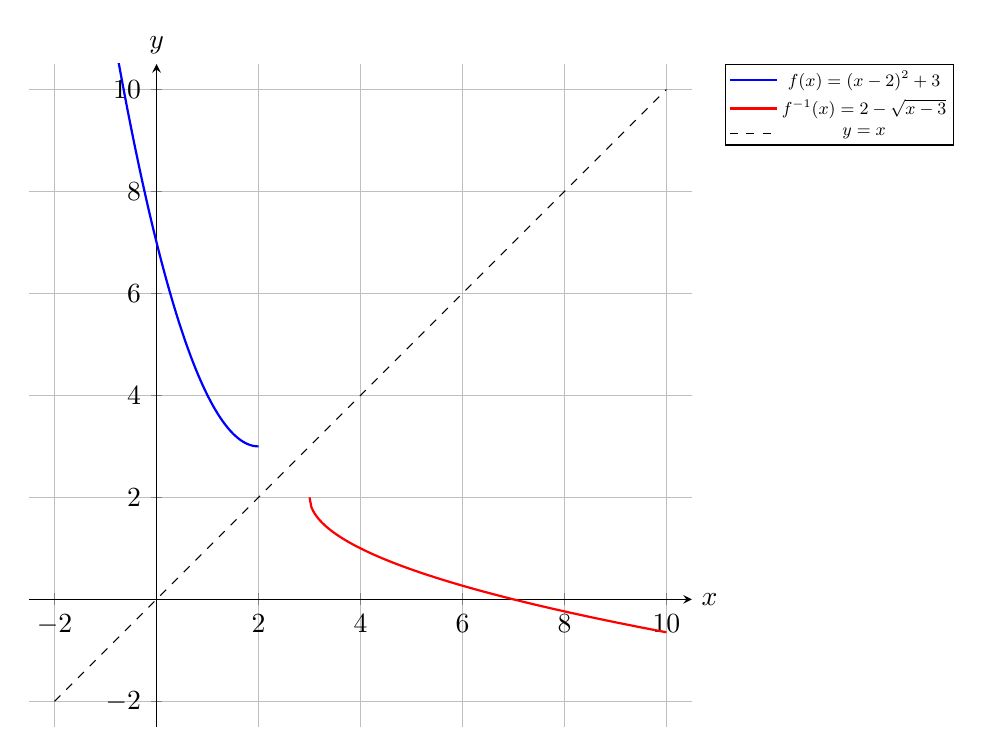
\begin{tikzpicture}
                            \begin{axis}[
                                    axis lines = middle,
                                    xlabel = $x$,
                                    ylabel = {$y$},
                                    xtick={-2,0,2,4,6,8,10},
                                    ytick={-2,0,2,4,6,8,10},
                                    ymin=-2.5, ymax=10.5,
                                    xmin=-2.5, xmax=10.5,
                                    grid=both,
                                    width=10cm,
                                    height=10cm,
                                    grid style={line width=.1pt, draw=gray!10},
                                    major grid style={line width=.2pt,draw=gray!50},
                                    x label style={anchor=west},
                                    y label style={anchor=south},
                                    samples=200,
                                    legend style={
                                            at={(1.05,1)},
                                            anchor=north west,
                                            font=\small,
                                            row sep=1pt,
                                            inner sep=1pt,
                                            nodes={scale=0.7}
                                        }
                                ]
                                \addplot[
                                    domain=-2:2,
                                    samples=200,
                                    color=blue,
                                    thick
                                ]
                                {(x-2)^2 + 3};
                                \addlegendentry{$f(x)=(x-2)^2+3$}

                                \addplot[
                                    domain=3:10,
                                    samples=200,
                                    color=red,
                                    thick
                                ]
                                {2 - sqrt(x-3)};
                                \addlegendentry{$f^{-1}(x)=2-\sqrt{x-3}$}

                                \addplot[
                                    domain=-2:10,
                                    samples=100,
                                    color=black,
                                    dashed
                                ]
                                {x};
                                \addlegendentry{$y=x$}
                            \end{axis}
                        \end{tikzpicture}
                    \end{center}
          \end{enumerate}
    \item Pada soal ini, kita cukup untuk menyamakan limit kiri dan limit kanan di $x=3$. Pada dasarnya kekontinuan di $x=3$ akan terpenuhi jika
          \begin{itemize}
              \item $f(3)$ terdefinisi,
              \item $\lim_{x \to 3} f(x)$ ada,
              \item $\lim_{x \to 3} f(x) = f(3)$.
          \end{itemize}
          Kita tahu bahwa $f(3)=3(3)-3=6$, sehingga $f(3)$ terdefinisi. Selanjutnya kita hitung limit kiri dan limit kanan di $x=3$,
          \begin{align*}
              \lim_{x \to 3^-} f(x) & = \lim_{x \to 3^-} (x^2 - k) = 3^2 - k = 9 - k, \\
              \lim_{x \to 3^+} f(x) & = \lim_{x \to 3^+} (3x - 3) = 3(3) - 3 = 6.
          \end{align*}
          Agar limit kiri dan limit kanan sama, maka
          \begin{align*}
              9 - k & = 6  \\
              k     & = 3.
          \end{align*}
          Dengan demikian, nilai $k$ agar $f(x)$ kontinu di $x=3$ adalah $k=3$.
    \item Fungsi tersebut dapat kita sederhanakan bentuknya menjadi
          \begin{align*}
              f(x) & = \sqrt{\frac{(3x+1)^3}{2x}} = \frac{(3x+1)^{3/2}}{(2x)^{1/2}} = \frac{(3x+1)^{3/2}}{\sqrt{2}\sqrt{x}} = \frac{1}{\sqrt{2}}(3x+1)^{3/2} x^{-1/2}.
          \end{align*}
          Untuk turunannya dapat kita gunakan aturan perkalian dan aturan rantai,
          \begin{align*}
              f'(x) & = \frac{1}{\sqrt{2}} \left[ \frac{3}{2}(3x+1)^{1/2} \cdot 3 \cdot x^{-1/2} + (3x+1)^{3/2} \cdot \left(-\frac{1}{2}\right) x^{-3/2} \right] \\
                    & = \frac{1}{\sqrt{2}} \left[ \frac{9}{2}(3x+1)^{1/2} x^{-1/2} - \frac{1}{2}(3x+1)^{3/2} x^{-3/2} \right]                                    \\
                    & = \frac{1}{2\sqrt{2}} \left[ 9(3x+1)^{1/2} x^{-1/2} - (3x+1)^{3/2} x^{-3/2} \right]                                                        \\
                    & = \frac{1}{2\sqrt{2}} (3x+1)^{1/2} x^{-3/2} [9x - (3x+1)]                                                                                  \\
                    & = \frac{1}{2\sqrt{2}} (3x+1)^{1/2} x^{-3/2} (6x - 1).
          \end{align*}
          Dengan demikian, turunan dari $f(x)$ adalah
          \[
              f'(x) = \frac{\sqrt{3x+1}\,(6x - 1)}{2x\sqrt{2x}}.
          \]
\end{enumerate}

\newpage
\renewcommand{\arraystretch}{1}
\fancyhead{}
\fancyfoot{}
\fancyhead[r]{}
\fancyhead[l]{\fbox{\large{\textbf{SKPB - ITS}}}}
\renewcommand{\headrulewidth}{0pt}
\renewcommand{\footrulewidth}{0pt}
\begin{center}
    {\underline{\textbf{\MakeUppercase{Evaluasi Tengah Semester Bersama Genap 2024/2025}}}}
\end{center}

\begin{center}
    \begin{tabular}{lcl}
        Mata kuliah/SKS & : & Kalkulus 1 ( SM234101 ) / 3 SKS \\
        Hari, Tanggal   & : & Kamis, 17 Oktober 2024          \\
        Waktu           & : & 11.00-12.40 WIB (100 menit)     \\
        Sifat           & : & Tertutup                        \\
        Kelas           & : & 20-33, 105, 106
    \end{tabular}
\end{center}

\noindent\rule{\textwidth}{2.pt}

\setlength{\parindent}{5pt}
\setlength{\parindent}{5pt}
\centering{Tuliskan: Nama, NRP, dan Nomor Kelas pada lembar jawaban Anda.}
\setlength{\parindent}{5pt}
\par \textbf{\small\MakeUppercase{dilarang membawa/menggunakan kalkulator dan alat komunikasi}}
\centering{\textbf{\MakeUppercase{dilarang memberikan/menerima jawaban selama ujian}}}
\par \centering{\textbf{"Setiap tindak kecurangan akan mendapat sanksi akademik."}}
\noindent\rule{\textwidth}{2.pt}

\begin{table}[h]
    \centering
    ETS Mengukur Kemampuan
    \begin{tabular}{|c|m{11cm}|c|c|}
        \hline
        CPL & CPMK                                                                                      & SOAL & BOBOT (\%) \\ \hline
        \multirow{5}{*}{2}
            & CPMK-1 Mampu menyelesaikan persamaan dan pertidaksamaan serta menssketsa grafik persamaan & 1    & 20         \\ \cline{2-4}
            & \multirow{4}{*}{CPMK-2 Mampu menentukan kekontinuan fungsi dan turunannya}                & 2    & 20         \\\cline{3-4}
            &                                                                                           & 3    & 20         \\ \cline{3-4}
            &                                                                                           & 4    & 20         \\ \cline{3-4}
            &                                                                                           & 5    & 20         \\ \hline
    \end{tabular}
\end{table}
{\centering\textbf{SOAL}}
% SOAL DI SINI YAA
\begin{enumerate}
    \item Dapatkan himpunan penyelesaian dari
          \[
              -1 \leq |2 - x| < 3.
          \]

    \item Diberikan $f(x) = \sqrt{25 - x^2}$ dan $g(x) = \dfrac{1}{x^2}$.
          \begin{enumerate}
              \item Dapatkan domain $f(x)$ dan $g(x)$.
              \item Dapatkan $(g \circ f)(x)$ dan domain $(g \circ f)(x)$.
          \end{enumerate}

    \item Diberikan $f(x) = \sqrt{4 - x^2}$.
          \begin{enumerate}
              \item Tentukan domain dari $f(x)$ sehingga inversnya ada.
              \item Dapatkan $f^{-1}(x)$ beserta domainnya.
          \end{enumerate}

    \item Diberikan fungsi
          \[
              f(x) =
              \begin{cases}
                  \dfrac{4 - x}{2 - \sqrt{x}}, & x \neq 4, \\[1em]
                  6,                           & x = 4,
              \end{cases}
          \]
          selidiki kekontinuan $f(x)$ di $x = 4$.

    \item Dapatkan $f''(x)$ dimana
          $
              f(x) = 2x + \bigl( 2\sqrt{x} - 3 \bigr)^{-2}.
          $

\end{enumerate}

\fancyfoot{\begin{center}
        \rule{0.28\textwidth}{2.pt}$\quad$\textbf{Selamat Mengerjakan}$\quad$\rule{0.28\textwidth}{2.pt}
        \begin{quote}
            \centering
            \textit{``Jujur adalah kunci kesuksesan''}
        \end{quote}
    \end{center}}


\newpage
\fancyfoot{}
\fancyhead[L]{\textit{Solution By: \hyperlink{https://github.com/TetewHeroez}{Tetew}}}
% \fancyfoot[R]{\animategraphics[autoplay,loop,width=0.1\textwidth]{15}{Kuru Kuru Herta/kuru kuru-}{0}{5}}
{\centering\textbf{SOLUSI}}
\renewcommand{\arraystretch}{1.5}
\renewcommand{\headrulewidth}{1pt}
\begin{enumerate}
    \item Karena nilai mutlak selalu bernilai positif, maka tidak perlu kita tinjau untuk kasus $-1 \leq |2 - x|$. Sehingga kita hanya perlu menyelesaikan pertidaksamaan $|2 - x| < 3$. Berdasarkan definisi nilai mutlak, maka
          \begin{align*}
              |2 - x| < 3 & \iff -3 < 2 - x < 3      \\
                          & \iff -3 - 2 < -x < 3 - 2 \\
                          & \iff -5 < -x < 1         \\
                          & \iff 5 > x > -1          \\
                          & \iff -1 < x < 5.
          \end{align*}
          Dengan demikian, himpunan penyelesaian dari pertidaksamaan tersebut adalah $(-1,5)$.
    \item \begin{enumerate}
              \item Agar $f(x) = \sqrt{25 - x^2}$ terdefinisi, maka $25 - x^2 \geq 0 \implies x^2 \leq 25 \implies -5 \leq x \leq 5$. Dengan demikian, domain dari $f$ adalah $\mathcal{D}_f = [-5,5]$. Sedangkan untuk $g(x) = \dfrac{1}{x^2}$, agar terdefinisi maka $x^2 \neq 0 \implies x \neq 0$. Dengan demikian, domain dari $g$ adalah $\mathcal{D}_g = \R \setminus \{0\}=\{x \in \R \,|\, x \ne 0\}$.
              \item \begin{align*}
                        (g \circ f)(x)  = g(f(x))
                        = g(\sqrt{25 - x^2})
                        = \frac{1}{(\sqrt{25 - x^2})^2}
                        = \frac{1}{25 - x^2}.
                    \end{align*}
                    Menurut definisi domain komposisi fungsi, maka
                    \begin{align*}
                        \mathcal{D}_{g \circ f} & = \{x \in \mathcal{D}_f \,|\, f(x) \in \mathcal{D}_g\}        \\
                                                & = \{x \in [-5,5] \,|\, \sqrt{25 - x^2} \in \R\setminus\{0\}\} \\
                                                & = \{x \in [-5,5] \,|\, 25 - x^2 \ne 0\}                       \\
                                                & = \{x \in [-5,5] \,|\, x^2 \ne 25\}                           \\
                                                & = \{x \in [-5,5] \,|\, x \ne 5\text{ dan } x \ne -5\}         \\
                                                & = (-5,5).
                    \end{align*}
                    Jadi domain dari $(g \circ f)(x)$ adalah $\mathcal{D}_{g \circ f} = (-5,5)$.
          \end{enumerate}
    \item \begin{enumerate}
              \item Agar $f(x) = \sqrt{4 - x^2}$ mempunyai invers, maka kita perlu membatasi domainnya pada salah satu sisi sumbu simetri yaitu $x=0$. Sehingga domain $f$ agar $f^{-1}$ ada adalah $\mathcal{D}_f = [0,2]$ atau $\mathcal{D}_f = [-2,0]$.
              \item Tukar $y = f(x)$ menjadi $x = f(y)$, sehingga
                    \begin{align*}
                        x                          & = \sqrt{4 - y^2}                           \\
                        x^2                        & = 4 - y^2                                  \\
                        y^2                        & = 4 - x^2                                  \\
                        y                          & = \pm\sqrt{4 - x^2}                        \\
                        f^{-1}(x) = \sqrt{4 - x^2} & \text{ atau } f^{-1}(x) = -\sqrt{4 - x^2}.
                    \end{align*}
                    Selanjutnya kita tahu bahwa $\mathcal{D}_{f^{-1}} = \mathcal{R}_f$. Jika kita ambil $\mathcal{D}_f = [0,2]$, maka $\mathcal{R}_f = [0,2]$ sehingga $\mathcal{D}_{f^{-1}} = [0,2]$ dan $f^{-1}(x) = \sqrt{4 - x^2}$.
                    Namun jika kita ambil $\mathcal{D}_f = [-2,0]$, maka $\mathcal{R}_f = [0,2]$ sehingga $\mathcal{D}_{f^{-1}} = [0,2]$ dan $f^{-1}(x) = -\sqrt{4 - x^2}$.
          \end{enumerate}
    \item Pada soal ini, kita cukup untuk menyamakan limit kiri dan limit kanan di $x=4$. Pada dasarnya kekontinuan di $x=4$ akan terpenuhi jika
          \begin{itemize}
              \item $f(4)$ terdefinisi,
              \item $\lim_{x \to 4} f(x)$ ada,
              \item $\lim_{x \to 4} f(x) = f(4)$.
          \end{itemize}
          Kita tahu bahwa $f(4)=6$, sehingga $f(4)$ terdefinisi. Selanjutnya kita hitung limit kiri dan limit kanan di $x=4$,
          \begin{align*}
              \lim_{x \to 4^-} f(x) & = \lim_{x \to 4^-} \frac{4 - x}{2 - \sqrt{x}} = \frac{4 - 4}{2 - \sqrt{4}} = \frac{0}{0}, \\
              \lim_{x \to 4^+} f(x) & = \lim_{x \to 4^+} 6 = 6.
          \end{align*}
          Karena limit kiri menghasilkan bentuk tak tentu $\frac{0}{0}$, maka kita perlu menyederhanakannya terlebih dahulu. Kita lakukan dengan cara mengalikan dengan bentuk sekawan dari penyebutnya, sehingga
          \begin{align*}
              \lim_{x \to 4^-} f(x) & = \lim_{x \to 4^-} \frac{4 - x}{2 - \sqrt{x}} \cdot \frac{2 + \sqrt{x}}{2 + \sqrt{x}}      \\
                                    & = \lim_{x \to 4^-} \frac{(4 - x)(2 + \sqrt{x})}{(2 - \sqrt{x})(2 + \sqrt{x})}              \\
                                    & = \lim_{x \to 4^-} \frac{(4 - x)(2 + \sqrt{x})}{4 - x}                                     \\
                                    & = \lim_{x \to 4^-} (2 + \sqrt{x})                                                          \\
                                    & = 2 + \sqrt{4}                                                                        = 4.
          \end{align*}
          Karena limit kiri dan limit kanan tidak sama, maka fungsi tersebut tidak kontinu di $x=4$.
    \item Dengan aturan rantai dapat diperoleh
          \begin{align*}
              f'(x) & = \frac{d}{dx}\left(2x+(2\sqrt{x} - 3)^{-2}\right)                           \\
                    & =\frac{d}{dx}(2x)+\frac{d}{dx}((2\sqrt{x} - 3)^{-2})                         \\
                    & =2 + (-2)(2\sqrt{x} - 3)^{-3} \cdot \frac{d}{dx}(2\sqrt{x} - 3)              \\
                    & =2 + (-2)(2\sqrt{x} - 3)^{-3} \cdot \left(2 \cdot \frac{1}{2\sqrt{x}}\right) \\
                    & =2 - 2(2\sqrt{x} - 3)^{-3} \cdot x^{-1/2}
          \end{align*}
          Selanjutnya, kita hitung turunan kedua $f''(x)$ dengan aturan perkalian. Misalkan
          \begin{align*}
              u  = -2(2\sqrt{x} - 3)^{-3} & \implies u' = 6(2\sqrt{x} - 3)^{-4} \cdot \frac{1}{\sqrt{x}}, \\
              v  = x^{-1/2}               & \implies v' = - \frac{1}{2} x^{-3/2}.
          \end{align*}
          Dengan demikian, diperoleh
          \begin{align*}
              f''(x) & = \frac{d}{dx}\left(2 - 2(2\sqrt{x} - 3)^{-3} \cdot x^{-1/2}\right)                                                               \\
                     & = 0 + \frac{d}{dx}\left(u \cdot v\right)                                                                                          \\
                     & = u'v + uv'                                                                                                                       \\
                     & = 6(2\sqrt{x} - 3)^{-4} \cdot \frac{1}{\sqrt{x}} \cdot x^{-1/2} + -2(2\sqrt{x} - 3)^{-3} \cdot \left(-\frac{1}{2} x^{-3/2}\right) \\
                     & = 6(2\sqrt{x} - 3)^{-4} x^{-1} + (2\sqrt{x} - 3)^{-3} x^{-3/2}.
          \end{align*}
\end{enumerate}

\newpage
\renewcommand{\arraystretch}{1}
\fancyhead{}
\fancyfoot{}
\fancyhead[r]{}
\fancyhead[l]{\fbox{\large{\textbf{SKPB - ITS}}}}
\renewcommand{\headrulewidth}{0pt}
\renewcommand{\footrulewidth}{0pt}
\begin{center}
    {\underline{\textbf{\MakeUppercase{Evaluasi Tengah Semester Bersama Genap 2024/2025}}}}
\end{center}

\begin{center}
    \begin{tabular}{lcl}
        Mata kuliah/SKS & : & Kalkulus 1 ( SM234101 ) / 3 SKS \\
        Hari, Tanggal   & : & Kamis, 17 Oktober 2024          \\
        Waktu           & : & 13.30-15.10 WIB (100 menit)     \\
        Sifat           & : & Tertutup                        \\
        Kelas           & : & 34-46, 107, 108
    \end{tabular}
\end{center}

\noindent\rule{\textwidth}{2.pt}

\setlength{\parindent}{5pt}
\setlength{\parindent}{5pt}
\centering{Tuliskan: Nama, NRP, dan Nomor Kelas pada lembar jawaban Anda.}
\setlength{\parindent}{5pt}
\par \textbf{\small\MakeUppercase{dilarang membawa/menggunakan kalkulator dan alat komunikasi}}
\centering{\textbf{\MakeUppercase{dilarang memberikan/menerima jawaban selama ujian}}}
\par \centering{\textbf{"Setiap tindak kecurangan akan mendapat sanksi akademik."}}
\noindent\rule{\textwidth}{2.pt}

\begin{table}[h]
    \centering
    ETS Mengukur Kemampuan
    \begin{tabular}{|c|m{11cm}|c|c|}
        \hline
        CPL & CPMK                                                                                      & SOAL & BOBOT (\%) \\ \hline
        \multirow{5}{*}{2}
            & CPMK-1 Mampu menyelesaikan persamaan dan pertidaksamaan serta menssketsa grafik persamaan & 1    & 20         \\ \cline{2-4}
            & \multirow{4}{*}{CPMK-2 Mampu menentukan kekontinuan fungsi dan turunannya}                & 2    & 20         \\\cline{3-4}
            &                                                                                           & 3    & 20         \\ \cline{3-4}
            &                                                                                           & 4    & 20         \\ \cline{3-4}
            &                                                                                           & 5    & 20         \\ \hline
    \end{tabular}
\end{table}
{\centering\textbf{SOAL}}
% SOAL DI SINI YAA
\begin{enumerate}
    \item Diberikan titik $A(1,1)$, $B(4,2)$ dan $C(2,6)$. Tentukan jarak dari titik $C$ ke garis yang melalui titik $A$ dan $B$.

    \item Diberikan $f(x) = x - 4$, untuk $x \geq 4$ dan $g(x) = \sqrt{4 - x^2}$.
          \begin{enumerate}
              \item Dapatkan domain $f(x)$ dan $g(x)$.
              \item Tentukan $(g \circ f)(x)$ dan domain $(g \circ f)(x)$.
          \end{enumerate}

    \item Diberikan fungsi $f(x) = \sqrt{2x - x^2}, \; 0 \leq x \leq 1$.
          \begin{enumerate}
              \item Tentukan $f^{-1}(x)$ beserta domainnya.
              \item Gambarkan grafik $f(x)$ dan $f^{-1}(x)$ dalam satu bidang koordinat.
          \end{enumerate}

    \item Hitunglah
          $\displaystyle
              \lim_{x \to 2} \frac{\sqrt{x^2 + 5} - 3}{x - 2}.
          $

    \item Diketahui persamaan garis singgung kurva $y^2 - xy = -2$ di titik $(a,b)$ sejajar dengan kurva $y = -x$.
          Dapatkan titik $(a,b)$.

\end{enumerate}

\fancyfoot{\begin{center}
        \rule{0.28\textwidth}{2.pt}$\quad$\textbf{Selamat Mengerjakan}$\quad$\rule{0.28\textwidth}{2.pt}
        \begin{quote}
            \centering
            \textit{``Jujur adalah kunci kesuksesan''}
        \end{quote}
    \end{center}}


\newpage
\fancyfoot{}
\fancyhead[L]{\textit{Solution By: \hyperlink{https://github.com/TetewHeroez}{Tetew}}}
% \fancyfoot[R]{\animategraphics[autoplay,loop,width=0.1\textwidth]{15}{Kuru Kuru Herta/kuru kuru-}{0}{5}}
{\centering\textbf{SOLUSI}}
\renewcommand{\arraystretch}{1.5}
\renewcommand{\headrulewidth}{1pt}
\begin{enumerate}
    \item Diketahui titik $A(1,1)$, $B(4,2)$ dan $C(2,6)$. Pertama kita cari persamaan garis yang melalui titik $A$ dan $B$. Gradien garis tersebut adalah
          \[
              m = \frac{y_2 - y_1}{x_2 - x_1} = \frac{2 - 1}{4 - 1} = \frac{1}{3}.
          \]
          Dengan menggunakan titik $A(1,1)$, maka persamaan garisnya adalah
          \begin{align*}
              y - y_1 & = m(x - x_1)         \\
              y - 1   & = \frac{1}{3}(x - 1) \\
              3y - 3  & = x - 1              \\
              x - 3y  & = -2.
          \end{align*}
          Dengan demikian, persamaan garis yang melalui titik $A$ dan $B$ adalah $x - 3y + 2 = 0$. Selanjutnya kita cari jarak dari titik $C(2,6)$ ke garis tersebut dengan rumus jarak titik ke garis,
          \begin{align*}
              d & = \frac{|Ax_0 + By_0 + C|}{\sqrt{A^2 + B^2}}       = \frac{|1(2) + (-3)(6) + 2|}{\sqrt{1^2 + (-3)^2}} = \frac{|-16|}{\sqrt{1 + 9}} = \frac{16}{\sqrt{10}}                             = \frac{16\sqrt{10}}{10}                            = \frac{8\sqrt{10}}{5}.
          \end{align*}
          Dengan demikian, jarak dari titik $C$ ke garis yang melalui titik $A$ dan $B$ adalah $\dfrac{8\sqrt{10}}{5}$ satuan.
    \item \begin{enumerate}
              \item Ingat bahwa fungsi polinomial terdefinisi di semua bilangan real, namun jika dalam soal diberikan batasan domain, maka kita ikuti batasan tersebut. Sehingga domain dari $f(x) = x - 4$ adalah $\mathcal{D}_f = [4,\infty)$. Sedangkan agar $g(x) = \sqrt{4 - x^2}$ terdefinisi, maka
                    \[
                        4 - x^2 \geq 0 \implies x^2 \leq 4 \implies -2 \leq x \leq 2.
                    \]
                    Dengan demikian, domain dari $g$ adalah $\mathcal{D}_g = [-2,2]$.
              \item \begin{align*}
                        (g \circ f)(x)  = g(f(x))
                        = g(x - 4)
                        = \sqrt{4 - (x - 4)^2}
                        = \sqrt{4 - (x^2 - 8x + 16)}
                        = \sqrt{-x^2 + 8x - 12}.
                    \end{align*}
                    Menurut definisi domain komposisi fungsi, maka
                    \begin{align*}
                        \mathcal{D}_{g \circ f} & = \{x \in \mathcal{D}_f \,|\, f(x) \in \mathcal{D}_g\} \\
                                                & = \{x \in [4,\infty) \,|\, x - 4 \in [-2,2]\}          \\
                                                & = \{x \geq 4 \,|\, -2 \leq x - 4 \leq 2\}              \\
                                                & = \{x \geq 4 \,|\, 2 \leq x \leq 6\}                   \\
                                                & = [4,6].
                    \end{align*}
                    Jadi domain dari $(g \circ f)(x)$ adalah $\mathcal{D}_{
                            g \circ f
                        } = [4,6]$.
          \end{enumerate}
    \item \begin{enumerate}
              \item Sebelum mencari ekspresi fungsi inversnya dapat kita tinjau bahwa domain $f$ adalah $\mathcal{D}_f = [0,1]$ dan range $f$ adalah $\mathcal{R}_f = [0,1]$. Sehingga domain dari $f^{-1}$ adalah $\mathcal{D}_{f^{-1}} = \mathcal{R}_f = [0,1]$.
                    Tukar $y = f(x)$ menjadi $x = f(y)$, sehingga
                    \begin{align*}
                        x            & = \sqrt{2y - y^2}      \\
                        x^2          & = 2y - y^2             \\
                        y^2 - 2y     & = -x^2                 \\
                        y^2 - 2y + 1 & = -x^2 + 1             \\
                        (y - 1)^2    & = 1 - x^2              \\
                        y - 1        & = \pm\sqrt{1 - x^2}    \\
                        y            & = 1 \pm \sqrt{1 - x^2}
                    \end{align*}
                    Karena $\mathcal{R}_{f^{-1}} = \mathcal{D}_f = [0,1]$, maka haruslah kita ambil $f^{-1}(x) = 1 - \sqrt{1 - x^2}$.
              \item \begin{center}
                        \begin{tikzpicture}
                            \begin{axis}[
                                    axis lines=middle,
                                    xlabel={$x$},
                                    ylabel={$y$},
                                    xmin=-0.5, xmax=1.5,
                                    ymin=-0.5, ymax=1.5,
                                    xtick={0,1},
                                    ytick={0,1},
                                    grid=both,
                                    grid style={line width=.1pt, draw=gray!10},
                                    major grid style={line width=.2pt,draw=gray!50},
                                    width=10cm,
                                    height=10cm,
                                    legend style={
                                            at={(1,1)},
                                            anchor=north west,
                                            font=\small,
                                            row sep=1pt,
                                            inner sep=1pt,
                                            nodes={scale=0.7}
                                        }
                                ]
                                \addplot[
                                    domain=0:1,
                                    samples=200,
                                    color=blue,
                                    thick
                                ]
                                {sqrt(2*x - x^2)};
                                \addlegendentry{$f(x)=\sqrt{2x - x^2}$}

                                \addplot[
                                    domain=0:1,
                                    samples=200,
                                    color=red,
                                    thick
                                ]
                                {1 - sqrt(1 - x^2)};
                                \addlegendentry{$f^{-1}(x)=1 - \sqrt{1 - x^2}$}

                                \addplot[
                                    domain=-0.5:1.5,
                                    samples=100,
                                    color=black,
                                    dashed
                                ]
                                {x};
                                \addlegendentry{$y=x$}
                            \end{axis}
                        \end{tikzpicture}
                    \end{center}
          \end{enumerate}
    \item Untuk menghitung limit tersebut, kita kalikan dengan bentuk sekawan dari pembilangnya, sehingga
          \begin{align*}
              \lim_{x \to 2} \frac{\sqrt{x^2 + 5} - 3}{x - 2} & = \lim_{x \to 2} \frac{\sqrt{x^2 + 5} - 3}{x - 2} \cdot \frac{\sqrt{x^2 + 5} + 3}{\sqrt{x^2 + 5} + 3}                                                                                                                                                                                                                                                                          \\
                                                              & = \lim_{x \to 2} \frac{(x^2 + 5) - 9}{(x - 2)(\sqrt{x^2 + 5} + 3)}                                                                                                                                                                                                                                                                                                             \\
                                                              & = \lim_{x \to 2} \frac{x^2 - 4}{(x - 2)(\sqrt{x^2 + 5} + 3)}                                                                                                                                                                                                                                                                                                                   \\
                                                              & = \lim_{x \to 2} \frac{(x - 2)(x + 2)}{(x - 2)(\sqrt{x^2 + 5} + 3)}                                                                                                                                                                                                                                                                                                            \\
                                                              & = \lim_{x \to 2} \frac{x + 2}{\sqrt{x^2 + 5} + 3}                                                                                                                                                                                                                                                                                                                              \\
                                                              & = \frac{2 + 2}{\sqrt{2^2 + 5} + 3}                                                             = \frac{4}{\sqrt{9} + 3}                                                             = \frac{4}{3 + 3}                                                                     = \frac{4}{6}                                                                         = \frac{2}{3}.
          \end{align*}
          Dengan demikian, nilai limit tersebut adalah $\dfrac{2}{3}$.
    \item Diketahui persamaan garis singgung kurva $y^2 - xy = -2$ di titik $(a,b)$ sejajar dengan kurva $y = -x$. Pertama kita cari turunan implisit dari persamaan kurva tersebut,
          \begin{align*}
              y^2 - xy                                              & = -2                \\
              2y \frac{dy}{dx} - \left( x \frac{dy}{dx} + y \right) & = 0                 \\
              2y \frac{dy}{dx} - x \frac{dy}{dx}                    & = y                 \\
              (2y - x) \frac{dy}{dx}                                & = y                 \\
              \frac{dy}{dx}                                         & = \frac{y}{2y - x}.
          \end{align*}
          Karena garis singgung di titik $(a,b)$ sejajar dengan kurva $y = -x$, maka gradien garis singgung tersebut adalah $-1$. Sehingga
          \begin{align*}
              \left. \frac{dy}{dx} \right|_{(a,b)} & = -1      \\
              \frac{b}{2b - a}                     & = -1      \\
              b                                    & = -2b + a \\
              3b                                   & = a       \\
              a                                    & = 3b.
          \end{align*}
          Selanjutnya kita substitusi $a=3b$ ke dalam persamaan kurva, sehingga
          \begin{align*}
              b^2 - (3b)b & = -2     \\
              b^2 - 3b^2  & = -2     \\
              -2b^2       & = -2     \\
              b^2         & = 1      \\
              b           & = \pm 1.
          \end{align*}
          Jika $b=1$, maka $a=3(1)=3$. Jika $b=-1$, maka $a=3(-1)=-3$. Dengan demikian, titik $(a,b)$ yang dimaksud adalah $(3,1)$ dan $(-3,-1)$.
\end{enumerate}

\newpage
\renewcommand{\arraystretch}{1}
\fancyhead{}
\fancyfoot{}
\fancyhead[r]{}
\fancyhead[l]{\fbox{\large{\textbf{SKPB - ITS}}}}
\renewcommand{\headrulewidth}{0pt}
\renewcommand{\footrulewidth}{0pt}
\begin{center}
    {\underline{\textbf{\MakeUppercase{Evaluasi Tengah Semester Bersama Genap 2024/2025}}}}
\end{center}

\begin{center}
    \begin{tabular}{lcl}
        Mata kuliah/SKS & : & Kalkulus 1 ( SM234101 ) / 3 SKS \\
        Hari, Tanggal   & : & Kamis, 17 Oktober 2024          \\
        Waktu           & : & 09.00-10.40 WIB (100 menit)     \\
        Sifat           & : & Tertutup                        \\
        Kelas           & : & 47-59, 111
    \end{tabular}
\end{center}

\noindent\rule{\textwidth}{2.pt}

\setlength{\parindent}{5pt}
\setlength{\parindent}{5pt}
\centering{Tuliskan: Nama, NRP, dan Nomor Kelas pada lembar jawaban Anda.}
\setlength{\parindent}{5pt}
\par \textbf{\small\MakeUppercase{dilarang membawa/menggunakan kalkulator dan alat komunikasi}}
\centering{\textbf{\MakeUppercase{dilarang memberikan/menerima jawaban selama ujian}}}
\par \centering{\textbf{"Setiap tindak kecurangan akan mendapat sanksi akademik."}}
\noindent\rule{\textwidth}{2.pt}

\begin{table}[h]
    \centering
    ETS Mengukur Kemampuan
    \begin{tabular}{|c|m{11cm}|c|c|}
        \hline
        CPL & CPMK                                                                                      & SOAL & BOBOT (\%) \\ \hline
        \multirow{5}{*}{2}
            & CPMK-1 Mampu menyelesaikan persamaan dan pertidaksamaan serta menssketsa grafik persamaan & 1    & 20         \\ \cline{2-4}
            & \multirow{4}{*}{CPMK-2 Mampu menentukan kekontinuan fungsi dan turunannya}                & 2    & 20         \\\cline{3-4}
            &                                                                                           & 3    & 20         \\ \cline{3-4}
            &                                                                                           & 4    & 20         \\ \cline{3-4}
            &                                                                                           & 5    & 20         \\ \hline
    \end{tabular}
\end{table}
{\centering\textbf{SOAL}}
% SOAL DI SINI YAA
\begin{enumerate}
    \item Dapatkan himpunan penyelesaian dari
          $\displaystyle
              \frac{x}{|2x - 5|} > 5.
          $

    \item Diberikan $f(x) = \sqrt{x - 3}$ dan $g(x) = 1 + \sqrt{x - 5}$.
          \begin{enumerate}
              \item Dapatkan domain $f(x)$ dan $g(x)$.
              \item Dapatkan $(f \circ g)(x)$ dan domain $(f \circ g)(x)$.
          \end{enumerate}

    \item Diberikan $f(x) = \sqrt[3]{x} - 1, \; x \geq 1$.
          \begin{enumerate}
              \item Dapatkan $f^{-1}(x)$ beserta domainnya.
              \item Sketsa $f(x)$ dan $f^{-1}(x)$ pada satu bidang koordinat.
          \end{enumerate}

    \item Hitunglah
          $\displaystyle
              \lim_{y \to \infty} \frac{2 - y}{\sqrt{7 + 4y^2}}.
          $

    \item Dapatkan persamaan garis singgung kurva
          $
              x^2 + y + \frac{y}{x} = \sqrt{x} + 2
          $
          di titik $(1,1)$.
\end{enumerate}


\fancyfoot{\begin{center}
        \rule{0.28\textwidth}{2.pt}$\quad$\textbf{Selamat Mengerjakan}$\quad$\rule{0.28\textwidth}{2.pt}
        \begin{quote}
            \centering
            \textit{``Jujur adalah kunci kesuksesan''}
        \end{quote}
    \end{center}}


\newpage
\fancyfoot{}
\fancyhead[L]{\textit{Solution By: \hyperlink{https://github.com/TetewHeroez}{Tetew}}}
% \fancyfoot[R]{\animategraphics[autoplay,loop,width=0.1\textwidth]{15}{Kuru Kuru Herta/kuru kuru-}{0}{5}}
{\centering\textbf{SOLUSI}}
\renewcommand{\arraystretch}{1.5}
\renewcommand{\headrulewidth}{1pt}
\begin{enumerate}
    \item Sebelum membagi kasus, perhatikan bahwa untuk $x = \frac{5}{2}$ akan menyebabkan penyebut menjadi nol. Sehingga dapat kita hiraukan nilai $x = \frac{5}{2}$ dari himpunan penyelesaian, maka yang perlu kita tinjau hanyalah
          \[
              x > 5|2x - 5|.\footnote{karena kita yakin bahwa $|2x - 5| \ne 0$, maka kita boleh mengalikan kedua ruas dengan $|2x - 5|$ tanpa mengubah arah pertidaksamaan.}
          \]
          Bagi kasus yaitu ketika $2x - 5 > 0$ dan $2x - 5 < 0$.\footnote{Kasus $2x - 5 = 0$ tidak perlu ditinjau karena akan menyebabkan penyebut menjadi nol.}
          \begin{itemize}
              \item Kasus $2x - 5 > 0 \implies x > \frac{5}{2}$. Diperoleh
                    \begin{align*}
                        x > 5|2x - 5| & \iff x > 5(2x - 5)     \\
                                      & \iff x > 10x - 25      \\
                                      & \iff -9x > -25         \\
                                      & \iff 9x < 25           \\
                                      & \iff x < \frac{25}{9}.
                    \end{align*}
                    Secara garis bilangan dapat diilustrasikan sebagai berikut,
                    \begin{center}
                        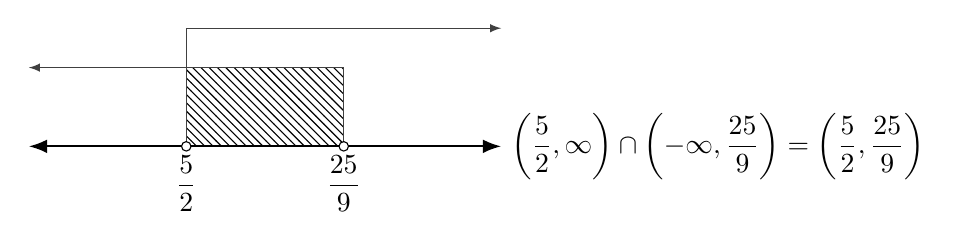
\begin{tikzpicture}
                            \draw[Latex-Latex,thick] (-2,-2) -- (4,-2) node[right]{$\left(\dfrac{5}{2},\infty\right)\cap\left(-\infty,\dfrac{25}{9}\right)=\left(\dfrac{5}{2},\dfrac{25}{9}\right)$};

                            \coordinate (A) at (2,-2);
                            \coordinate (B) at (0,-2);

                            \fill[pattern=north west lines] (B) -- (A)--(2,-1)--(0,-1)--cycle;

                            \draw[-latex,darkgray] (A) -- (2,-1) -- (-2,-1);
                            \draw[-latex,darkgray] (B) -- (0,-0.5) -- (4,-0.5);

                            \draw[fill=white] (A) circle (0.06) node[below]{$\dfrac{25}{9}$};
                            \draw[fill=white] (B) circle (0.06) node[below]{$\dfrac{5}{2}$};
                        \end{tikzpicture}
                    \end{center}
              \item Kasus $2x - 5 < 0 \implies x < \frac{5}{2}$.
                    Maka
                    \begin{align*}
                        x > 5|2x - 5| & \iff x < -5(2x - 5)     \\
                                      & \iff x < -10x + 25      \\
                                      & \iff 11x < 25           \\
                                      & \iff x < \frac{25}{11}.
                    \end{align*}
                    \begin{center}
                        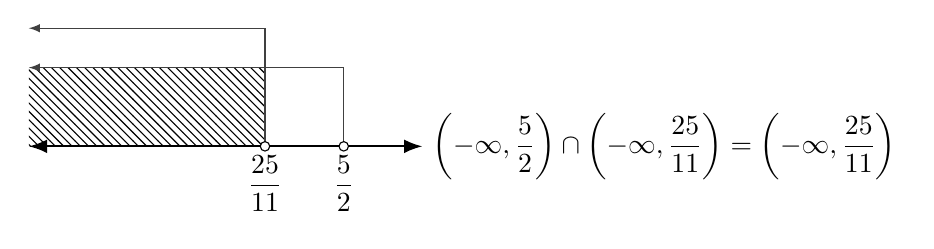
\begin{tikzpicture}
                            \draw[Latex-Latex,thick] (-3,-2) -- (2,-2) node[right]{$\left(-\infty,\dfrac{5}{2}\right)\cap\left(-\infty,\dfrac{25}{11}\right)=\left(-\infty,\dfrac{25}{11}\right)$};

                            \coordinate (A) at (1,-2);
                            \coordinate (B) at (0,-2);

                            \fill[pattern=north west lines] (B) --(0,-1)--(-3,-1)--(-3,-2);

                            \draw[-latex,darkgray] (A) -- (1,-1) -- (-3,-1);
                            \draw[-latex,darkgray] (B) -- (0,-0.5) -- (-3,-0.5);

                            \draw[fill=white] (A) circle (0.06) node[below]{$\dfrac{5}{2}$};
                            \draw[fill=white] (B) circle (0.06) node[below]{$\dfrac{25}{11}$};
                        \end{tikzpicture}
                    \end{center}
          \end{itemize}
          Dengan demikian, himpunan penyelesaian dari pertidaksamaan tersebut adalah
          \[
              \left(-\infty,\frac{25}{11}\right) \cup \left(\frac{5}{2},\frac{25}{9}\right).
          \]

    \item \begin{enumerate}
              \item Agar $f(x) = \sqrt{x - 3}$ terdefinisi, maka $x - 3 \geq 0 \implies x \geq 3$. Dengan demikian, domain dari $f$ adalah $\mathcal{D}_f = [3,\infty)$. Sedangkan untuk $g(x) = 1 + \sqrt{x - 5}$, agar terdefinisi maka $x - 5 \geq 0 \implies x \geq 5$. Dengan demikian, domain dari $g$ adalah $\mathcal{D}_g = [5,\infty)$.
              \item \begin{align*}
                        (f \circ g)(x)  = f(g(x))
                        = f(1 + \sqrt{x - 5})
                        = \sqrt{(1 + \sqrt{x - 5}) - 3}
                        = \sqrt{\sqrt{x - 5} - 2}.
                    \end{align*}
                    Menurut definisi domain komposisi fungsi, maka
                    \begin{align*}
                        \mathcal{D}_{f \circ g} & = \{x \in \mathcal{D}_g \,|\, g(x) \in \mathcal{D}_f\}       \\
                                                & = \{x \in [5,\infty) \,|\, 1 + \sqrt{x - 5} \in [3,\infty)\} \\
                                                & = \{x \geq 5 \,|\, 1 + \sqrt{x - 5} \geq 3\}                 \\
                                                & = \{x \geq 5 \,|\, \sqrt{x - 5} \geq 2\}                     \\
                                                & = \{x \geq 5 \,|\, x - 5 \geq 4\}                            \\
                                                & = \{x \geq 5 \,|\, x \geq 9\}                                \\
                                                & = [9,\infty).
                    \end{align*}
                    Jadi domain dari $(f \circ g)(x)$ adalah $\mathcal{D}_{f \circ g} = [9,\infty)$.
          \end{enumerate}
    \item \begin{enumerate}
              \item Sebelum mencari ekspresi fungsi inversnya dapat kita tinjau bahwa domain $f$ adalah $\mathcal{D}_f = [1,\infty)$ dan range $f$ adalah $\mathcal{R}_f = [0,\infty)$. Sehingga domain dari $f^{-1}$ adalah $\mathcal{D}_{f^{-1}} = \mathcal{R}_f = [0,\infty)$.
                    Tukar $y = f(x)$ menjadi $x = f(y)$, sehingga
                    \begin{align*}
                        x         & = \sqrt[3]{y} - 1 \\
                        x + 1     & = \sqrt[3]{y}     \\
                        (x + 1)^3 & = y               \\
                        f^{-1}(x) & = (x + 1)^3.
                    \end{align*}
              \item \begin{center}
                        \begin{tikzpicture}
                            \begin{axis}[
                                    axis lines=middle,
                                    xlabel={$x$},
                                    ylabel={$y$},
                                    xmin=-1, xmax=4,
                                    ymin=-1, ymax=4,
                                    xtick={0,1,2,3},
                                    ytick={0,1,2,3},
                                    grid=both,
                                    grid style={line width=.1pt, draw=gray!10},
                                    major grid style={line width=.2pt,draw=gray!50},
                                    width=10cm,
                                    height=10cm,
                                    legend style={
                                            at={(1,1)},
                                            anchor=north west,
                                            font=\small,
                                            row sep=1pt,
                                            inner sep=1pt,
                                            nodes={scale=0.7}
                                        }
                                ]
                                \addplot[
                                    domain=1:4,
                                    samples=200,
                                    color=blue,
                                    thick
                                ]
                                {x^(1/3) - 1};
                                \addlegendentry{$f(x)=\sqrt[3]{x} - 1$}

                                \addplot[
                                    domain=0:3,
                                    samples=200,
                                    color=red,
                                    thick
                                ]
                                {(x + 1)^3};
                                \addlegendentry{$f^{-1}(x)=(x + 1)^3$}

                                \addplot[
                                    domain=-1:4,
                                    samples=100,
                                    color=black,
                                    dashed
                                ]
                                {x};
                                \addlegendentry{$y=x$}
                            \end{axis}
                        \end{tikzpicture}
                    \end{center}
          \end{enumerate}
    \item  Untuk menghitung limit tersebut, kita bagi pembilang dan penyebut dengan $|y|$, sehingga
          \begin{align*}
              \lim_{y \to \infty} \frac{2 - y}{\sqrt{7 + 4y^2}} & = \lim_{y \to \infty} \frac{\frac{2 - y}{|y|}}{\frac{\sqrt{7 + 4y^2}}{|y|}}    = \lim_{y \to \infty} \frac{\frac{2}{|y|} - \frac{y}{|y|}}{\sqrt{\frac{7}{y^2} + 4}}
          \end{align*}
          Karena $y \to \infty$, maka $y > 0$ sehingga $|y| = y$. Oleh karena itu,
          \begin{align*}
              \lim_{y \to \infty} \frac{2 - y}{\sqrt{7 + 4y^2}} & = \lim_{y \to \infty} \frac{\frac{2}{y} - 1}{\sqrt{\frac{7}{y^2} + 4}}                                                                 = \frac{\lim_{y \to \infty} \left(\frac{2}{y} - 1\right)}{\lim_{y \to \infty} \sqrt{\frac{7}{y^2} + 4}}                                                                                 = \frac{0 - 1}{\sqrt{0 + 4}}                                                                                                     = \frac{-1}{\sqrt{4}}                                                                                                     = \frac{-1}{2}.
          \end{align*}
          Dengan demikian, nilai limit tersebut adalah $-\dfrac{1}{2}$.

    \item Pertama kita cari turunan implisit dari persamaan kurva tersebut,
          \begin{align*}
              x^2 + y + \frac{y}{x}                                              & = \sqrt{x} + 2            \\
              2x + \frac{dy}{dx} + \frac{\frac{dy}{dx} \cdot x - y \cdot 1}{x^2} & = \frac{1}{2\sqrt{x}} + 0 \\
              2x + \frac{dy}{dx} + \frac{x \frac{dy}{dx} - y}{x^2}               & = \frac{1}{2\sqrt{x}}     \\
              2x + \frac{dy}{dx} + \frac{\frac{dy}{dx}}{x} - \frac{y}{x^2}       & = \frac{1}{2\sqrt{x}}
          \end{align*}
          Selanjutnya kita substitusi titik $(1,1)$ ke dalam turunan tersebut, sehingga
          \begin{align*}
              2(1) + \left.\frac{dy}{dx}\right|_{(1,1)} + \frac{\left.\frac{dy}{dx}\right|_{(1,1)}}{1} - \frac{1}{1^2} & = \frac{1}{2\sqrt{1}} \\
              2 + \left.\frac{dy}{dx}\right|_{(1,1)} + \left.\frac{dy}{dx}\right|_{(1,1)} - 1                          & = \frac{1}{2}         \\
              1 + 2\left.\frac{dy}{dx}\right|_{(1,1)}                                                                  & = \frac{1}{2}         \\
              2\left.\frac{dy}{dx}\right|_{(1,1)}                                                                      & = -\frac{1}{2}        \\
              \left.\frac{dy}{dx}\right|_{(1,1)}                                                                       & = -\frac{1}{4}.
          \end{align*}
          Dengan demikian, gradien garis singgung di titik $(1,1)$ adalah $-\dfrac{1}{4}$. Sehingga persamaan garis singgungnya adalah
          \begin{align*}
              y - y_1 & = m(x - x_1)          \\
              y - 1   & = -\frac{1}{4}(x - 1) \\
              4y - 4  & = -x + 1              \\
              x + 4y  & = 5.
          \end{align*}
          Dengan demikian, persamaan garis singgung kurva di titik $(1,1)$ adalah $x + 4y = 5$.
\end{enumerate}
\end{document}